\chapter{Appendix}


\section{Overview of the cluster}
\begin{figure}[H]
    \centerline{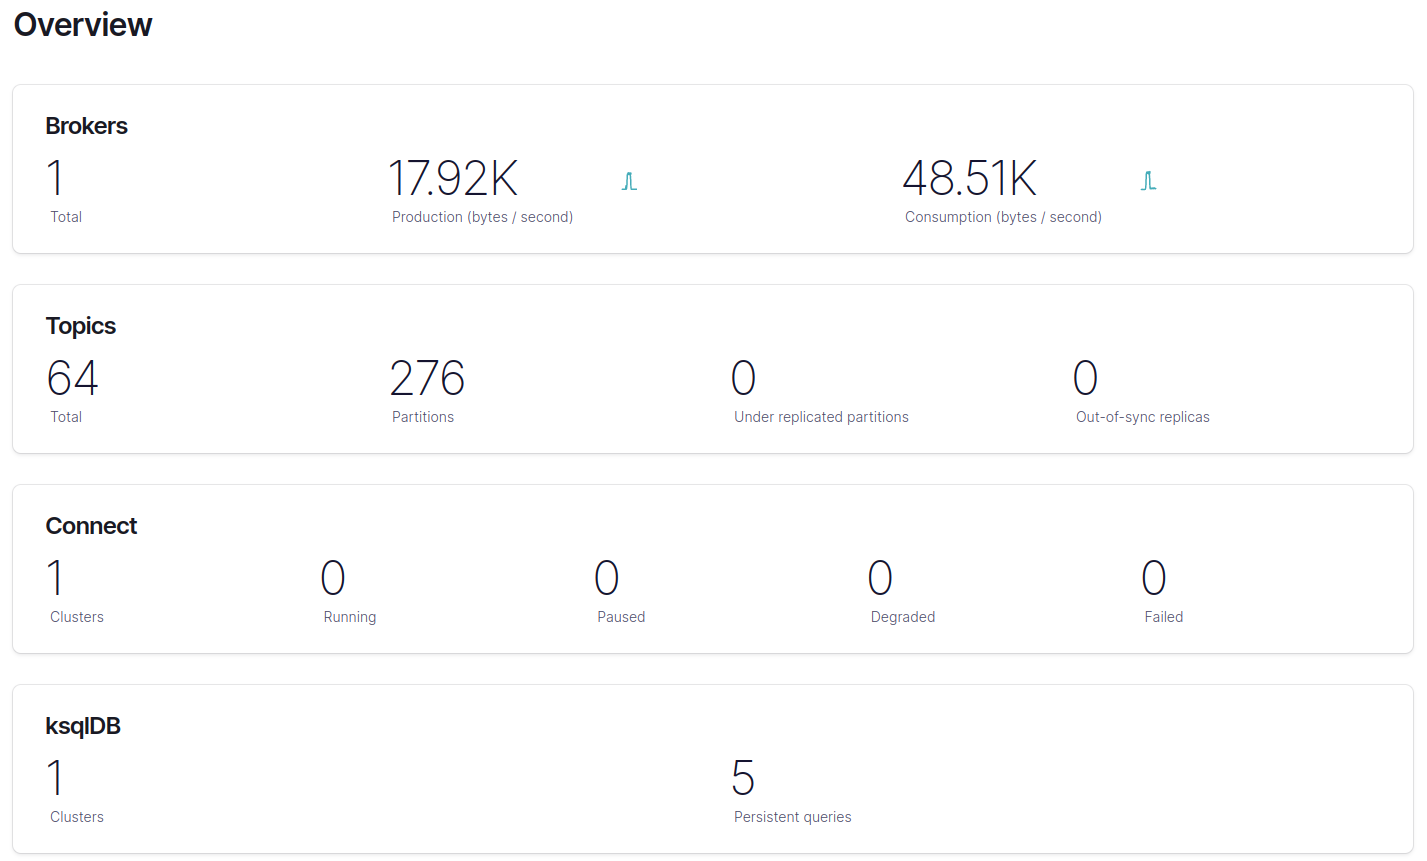
\includegraphics[scale=.3]{assets/appendices/overview.png}}
    \caption{Cluster overview  }
    \label{fig}
\end{figure}
* Shown number of topics include hidden internal topics on Cluster Overview
\section{The average end-to-end latency}
\begin{figure}[H]
    \centerline{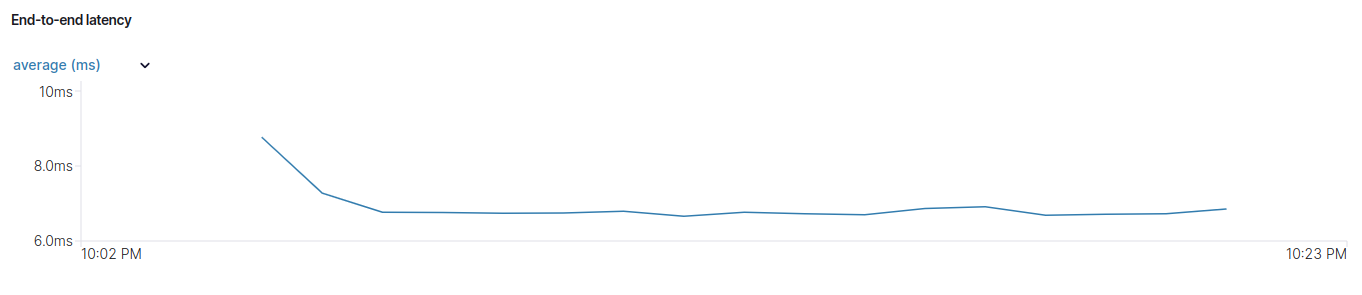
\includegraphics[scale=.4]{assets/appendices/average-end-to-end-latency.png}}
    \caption{The average end-to-end latency}
    \label{fig}
\end{figure}

\section{Throughput graph}
\begin{figure}[H]
    \centerline{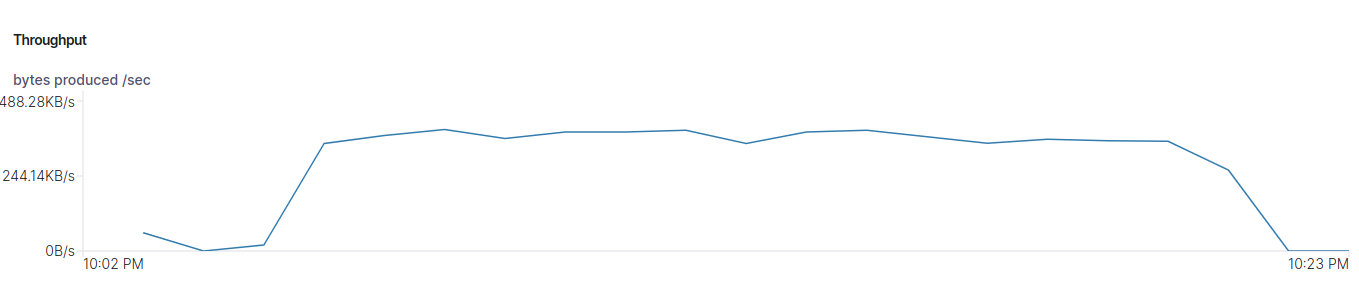
\includegraphics[scale=.4]{assets/appendices/throughput_graph.png}}
    \caption{Throughput graph}
    \label{fig}
\end{figure}

\section{Consumed throughput graph}
\begin{figure}[H]
    \centerline{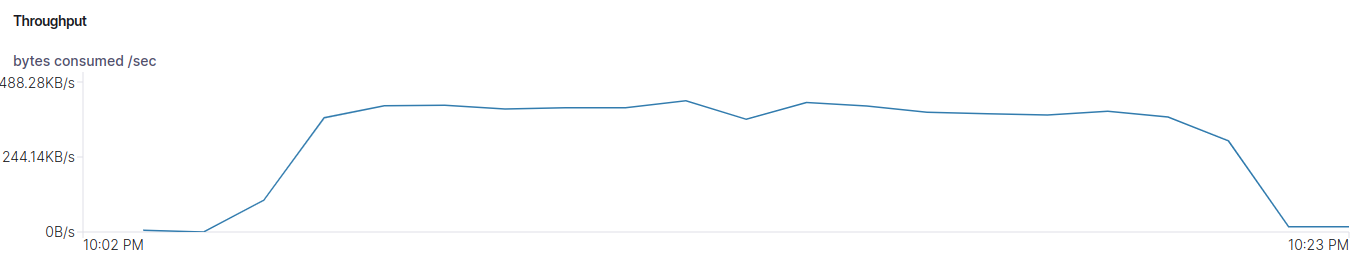
\includegraphics[scale=.4]{assets/appendices/throuhput-consumed.png}}
    \caption{Consumed throughput graph}
    \label{fig}
\end{figure}

\section{Topics}

\begin{figure}[H]
    \centerline{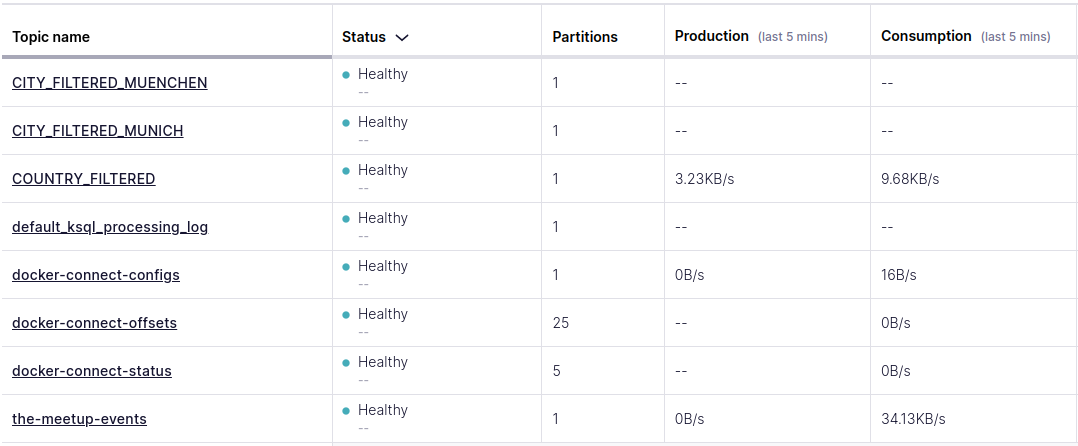
\includegraphics[scale=.4]{assets/appendices/topics-table.png}}
    \caption{Topics table}
    \label{fig}
\end{figure}

* Topics are automatically generated, topics which starts with `docker` and  `default` are internal topics.